\documentclass[final,paperwidth=36in,paperheight=48in,portrait,fontscale=0.36]{baposter}
% NIPS Workshops format

% Encoding.
\usepackage[utf8]{inputenc}
\usepackage[T1]{fontenc}

\usepackage{graphicx} % Required for including images
\usepackage{booktabs} % for professional tables
\usepackage{floatrow}
\usepackage{amsmath} % For typesetting math
\usepackage[font=small,labelfont=bf, justification=centering]{caption} % Required for specifying captions to tables and figures

\usepackage{multicol} % Required for multiple columns
\setlength{\columnsep}{1cm}
\setlength{\columnseprule}{0.5pt}
\usepackage{multirow}
\usepackage{graphicx}

% For gap between cmidrules.
\usepackage{array}
\newcolumntype{C}{@{\extracolsep{0.1cm}}c@{\extracolsep{0pt}}}%

\newcommand{\compresslist}{ % Define a command to reduce spacing within itemize/enumerate environments, this is used right after \begin{itemize} or \begin{enumerate}
\setlength{\itemsep}{1pt}
\setlength{\parskip}{0pt}
\setlength{\parsep}{0pt}
}

% Defines the color used for content box headers
\definecolor{lightblue}{cmyk}{0.83,0.24,0,0.16}

%%%%%%%%%%%%%%%%%%%%%%%%%%%%%%%%%%%%%%
% macros for the equations
\newcommand{\cw}{\mathbf{cw}}
\newcommand{\cc}{\mathbf{c}}
\newcommand{\kb}{\mathbf{k}}
\newcommand{\mem}{\mathbf{m}}
\newcommand{\rr}{\mathbf{r}}
%%%%%%%%%%%%%%%%%%%%%%%%%%%%%%%%%%%%%%

%%%%%%%%%%%%%%%%%%%%%%%%%%%%%%%%%%%%%%%%%%%%%%%%%%%%%%%%%%%%%%%%%%%%%%%%%%%%%%
%%% Begin of Document
%%%%%%%%%%%%%%%%%%%%%%%%%%%%%%%%%%%%%%%%%%%%%%%%%%%%%%%%%%%%%%%%%%%%%%%%%%%%%%
\frenchspacing

\begin{document}

\hyphenation{resolution occlusions}
%%
\begin{poster}%
  % Poster Options
  {
  % Show grid to help with alignment
  grid=false,
  % Column spacing
  colspacing=1em,
  % Color style
  bgColorOne=white,
  bgColorTwo=white,
  borderColor=lightblue,
  headerColorOne=black,
  headerColorTwo=lightblue,
  headerFontColor=white,
  boxColorOne=white,
  boxColorTwo=lightblue,
  % Format of textbox
  textborder=roundedleft,
%  textborder=faded,
  % Format of text header
  eyecatcher=true,
  headerborder=closed,
  columns=2,
  headerheight=3cm,
%  textfont=\sc, An example of changing the text font
  headershape=roundedright,
  headershade=shadelr,
  headerfont=\Large\bf\textsc, %Sans Serif
  textfont={\setlength{\parindent}{1.5em}\large},
  boxshade=plain,
%  background=shade-tb,
  background=plain,
  linewidth=1pt
  } 
  { % Left Eye Catcher - IBM logo
	
\includegraphics[width=4cm]{../img/ibm_research.png}
  } 
  % Title
  	{\bf\textsc{On transfer learning using a MAC model variant}\vspace{0.2em}}
  % Authors
  {
	\textbf{\null\hfill Vincent Marois \hfill T.S. Jayram \hfill Vincent Albouy \hfill Tomasz Kornuta \hfill\null}\\
	\textbf{\null\hfill Younes Bouhadjar \hfill Ahmet S. Ozcan \hfill\null}\\
	\texttt{\{vmarois,jayram,tkornut,byounes,asozcan\}@us.ibm.com, \{vincent.albouy\}@ibm.com}
  }
  { % Left Eye Catcher
  	
\includegraphics[width=4cm]{../img/arc_logo.png}
  }

%%%%%%%%%%%%%%%%%%%%%%%%%%%%%%%%%%%%%%%%%%%%%%%%%%%%%%%%%%%%%%%%%%%%%%%%%%%%%%%
\headerbox{Summary}{name=summary,column=0,row=0}{
\begin{itemize}
	\compresslist
	\item[$\bullet$] We introduce a simplified variant of the MAC model (\textit{Hudson and Manning, ICLR 2018}), which achieves comparable accuracy while training faster.
	\item[$\bullet$] We evaluate both models on CLEVR \& CoGenT, and show that, transfer learning with fine-tuning results in a 15 point increase in accuracy, matching the state of the art.
	\item[$\bullet$] We also demonstrate that improper fine-tuning can reduce a model's accuracy.
	
\end{itemize}

} %headerbox

\headerbox{The MAC Model ~\cite{hudson2018compositional}}{name=mac-model, column=0, below=summary}{
	\vspace{-10pt}
	\begin{figure}[H]
		\centering
		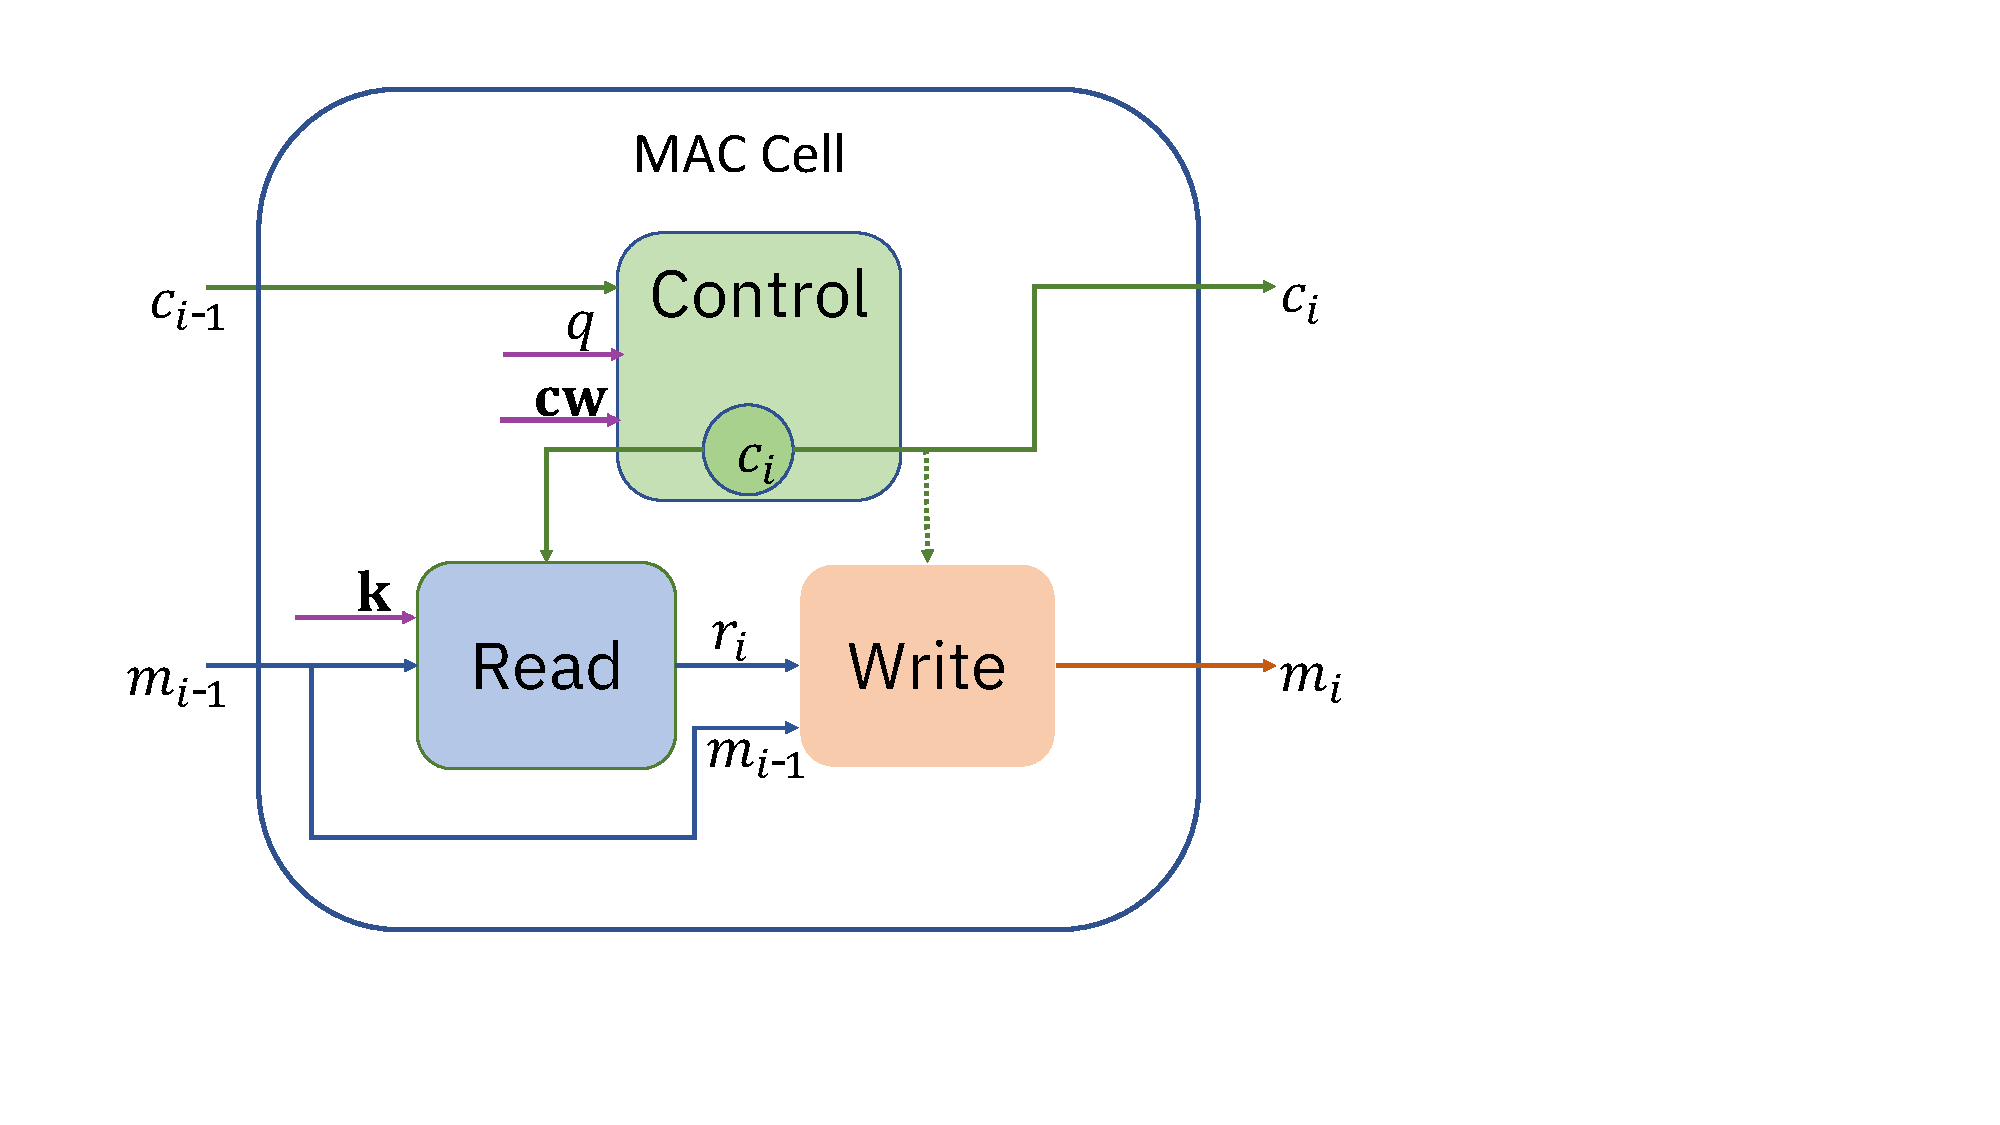
\includegraphics[width=0.33\textwidth]{../img/mac_cell.pdf}
		\caption{The MAC cell ~\cite{hudson2018compositional}.}
		\label{fig:mac_cell}
	\end{figure}
	\vspace{-20pt}
	\begin{itemize}
		\compresslist
		\item[$\bullet$] MAC network: a recurrent model performing sequential reasoning. At each step, it analyzes the question and shifts the attention over the image.
		\item[$\bullet$] Recurrent MAC cell: consists of a control unit, a read unit \& a write unit. The control unit updates the control state $c_i$ \& drives the attention over the question words.
		\item[$\bullet$] The read unit, guided by $c_i$ extracts information from the image. The write unit uses this information to update the memory state $m_i$.
	\end{itemize}
}

\headerbox{Simplified Mac Model (S-MAC)}{name=s-mac, column=0, below=mac-model}{
	
	Based on two heuristic simplifications:
	
	\begin{itemize}
		\compresslist
	    \item[$\bullet$] Taking the MAC cell equations as a whole, consecutive linear layers (with no activation in-between) can be combined as one linear layer.
		\item[$\bullet$] We assume that dimension-preserving linear layers are invertible so as to avoid information loss.
    \end{itemize}

	This allows, with a careful reorganization, to apply a single linear layer to the \textit{knowledge base} (feature map extracted from the image) prior to all the reasoning steps and work with this projection throughout the reasoning steps.\\

\makebox[\textwidth]{MAC  \\[5cm] S-MAC}\\
\noindent\textbf{Control unit:} The question $q$ is first made \emph{position-aware} in each reasoning step using an $i$-dependent projection: $q_i = U_i^{[d \times 2d]} q + b_i^{[d]}$.


\begin{multicols}{2}
	\noindent
	\begin{align*}
	&cq_i = W_{cq}^{[d \times 2d]} [c_{i-1}, q_i] + b_{cq}^{[d]}  \tag{c1} \\
	&ca_{is} = W_{ca}^{[1 \times d]} (cq_i \odot \cw_s) + b_{ca}^{[1]}
	\tag{c2.1}\\
	&cv_{is} = \textrm{softmax}(ca_{is}) \tag{c2.2}\\
	&\cc_i = \sum_s cv_{is} \, \cw_s  \tag{c2.3}
	\end{align*}
	\columnbreak
	{
		\begin{align*}
		&cq_i = W_{cq}^{[d \times d]} c_{i-1} + q_i  \tag{c1} \\
		&ca_{is} = W_{ca}^{[1 \times d]} (cq_i \odot \cw_s)  \tag{c2.1}\\
		&cv_{is} = \textrm{softmax}(ca_{is}) \tag{c2.2}\\
		&\cc_i = \sum_s cv_{is} \, \cw_s  \tag{c2.3}
		\end{align*}}
\end{multicols}

\vskip -0.6cm

\noindent\textbf{Read and write units:}
\begin{multicols}{2}
	\noindent
	\begin{align*}
	&I_{ihw} = (W_{m}^{[d \times d]} \mem_{i-1} + b_{m}^{[d]}) \\
	& \qquad \quad \odot (W_{k}^{[d \times d]} \kb_{hw} + b_{k}^{[d]}) \tag{r1} \\
	&I'_{ihw} =  W_{I'}^{[d \times 2d]} [I_{ihw},\kb_{hw}]  + b_{I'}^{[d]}  \tag{r2} \\
	&ra_{ihw} = W_{ra}^{[1 \times d]} (\cc_i \odot I'_{ihw}) + b_{ra}^{[1]} \tag{r3.1}\\
	&rv_{ihw} = \textrm{softmax}(ra_{ihw}) \tag{r3.2}\\
	&\rr_i = \sum_s rv_{ihw} \, \kb_{hw}  \tag{r3.3}\\
	&\mem_i = W_{rm}^{[d \times d]} [\rr_i, \mem_{i-1}]  + b_{rm}^{[d]} \tag{w1}	
	\end{align*}
	\columnbreak
	{
		\begin{align*}
		&I_{ihw} = m _{i-1} \odot k _{hw} \tag{r1} \\ 
		&I'_{ihw} = W_{I'}^{[d \times d]} I_{ihw} + b_{I'}^{[d]} + \kb_{hw} \tag{r2} \\
		&ra_{ihw} = W_{ra}^{[1 \times d]} (\cc_i \odot I'_{ihw})  \tag{r3.1}\\
		&rv_{ihw} = \textrm{softmax}(ra_{ihw}) \tag{r3.2}\\
		&\rr_i = \sum_s rv_{ihw} \, \kb_{hw}  \tag{r3.3}\\
		&\mem_i = W_{rm}^{[d \times 2d]} \rr_i + b_{rm}^{[d]} \tag{w1}
		\end{align*}}
\end{multicols}
	
\begin{table}[H]
	\centering
	\caption{Comparing the number of position-independent parameters between MAC \& S-MAC cells.}
	\begin{tabular}{llll}
		\toprule
		Model        & Read Unit               & Write Unit &  Control Unit         \\
		\midrule
		MAC   &  787,969 &  524,800        &    525,313    \\
		%\midrule
		simplified MAC & 263,168  & 262,656       &    263,168 \\
		\midrule
		Reduction by [\%]  & 67\%  &   50\%       &      50\%  \\
		\bottomrule
	\end{tabular}
	\label{tab:mac_cell_parameters}
\end{table}

}




\headerbox{Links}{name=links,column=0,below=s-mac}{
	\vspace{-15pt}
	\begin{minipage}[H]{0.4\textwidth}
		\begin{figure}[H]
			
\includegraphics[width=0.4\textwidth]{../img/doc_qr_code.png}
			\vspace{-10pt}
			\caption{Documentation.}
			\label{fig:qr_doc}
		\end{figure}
	\end{minipage}
	\hfill
	\begin{minipage}[H]{0.4\textwidth}
		\begin{figure}[H]
			
\includegraphics[width=0.4\textwidth]{../img/github_repo_qr_code.png}
			\vspace{-10pt}
			\caption{GitHub repo.}
			\label{fig:qr_github}
		\end{figure}
	\end{minipage}
}

	
	
	


\headerbox{Datasets - CLEVR and CoGenT}{name=dataset, column=1}{
The CLEVR task:
		\begin{figure}[H]
		\centering
		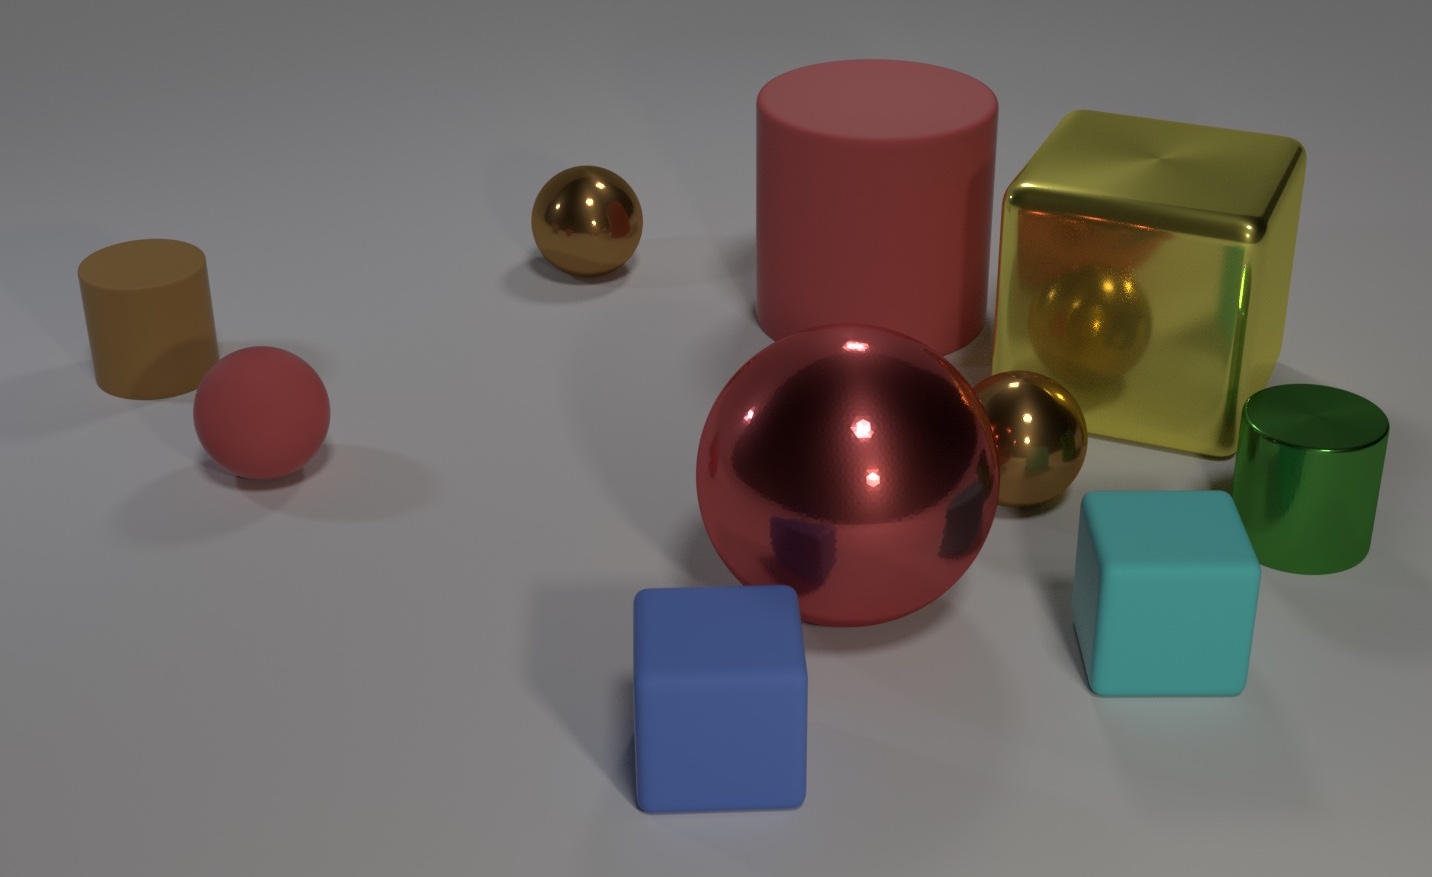
\includegraphics[width=0.31\textwidth]{../img/teaser.jpg}
	    \end{figure}
    
    
    \begin{description}
    	\centering
    	\item[$\cdot$] \textit{How many objects are either small cylinders or red things?}
    	
    \end{description}


   \begin{description}
   	\item[$\bullet$]Along with CLEVR, the authors~\cite{johnson2017clevr} introduced  CLEVR-CoGenT 
   	\item[$\bullet$] The goal is to evaluate how well the models can generalize, learn relations and compositional concepts.
   	\item[$\bullet$] This dataset is generated in the same way as CLEVR, with two conditions, A and B. as shown in Table 2.

   \end{description}

	\begin{table}[H]
		\centering
		\begin{tabular}{llll}
			\toprule
			Dataset        & Cubes              & Cylinders &  Spheres         \\
			\midrule
			CLEVR   &  any color &  any color        &    any color    \\
			CLEVR CoGenT A & gray / blue / brown / yellow  & red / green / purple / cyan       &    any color  \\
			CLEVR CoGenT B  & red / green / purple / cyan &   gray / blue / brown / yellow       &      any color  \\
			\bottomrule
		\end{tabular}
		\caption{Colors/shapes combinations present in CLEVR, CoGenT-A and CoGenT-B datasets.}
		\label{tab:cogent_conditions}
	\end{table}
	
}




\headerbox{Transfer Learning - Experiments}{name=transfer, column=1, below=dataset}{

CLEVR \& CoGenT accuracies for the MAC \& S-MAC models:
	\begin{table}[H]
	\centering
	\scalebox{1}{
	\begin{tabular}{lllllllll}
		\toprule
		\multirow{2}{*}{Model} & \multicolumn{3}{c}{Training} &  \multicolumn{2}{c}{Fine-tuning} & \multicolumn{2}{c}{Test} & \multirow{2}{*}{Row} \\
		\cmidrule{2-4} \cmidrule{5-6} \cmidrule{7-8} 
		& Dataset                & Time [h:m] & Acc [\%]          & Dataset & Acc [\%]  & Dataset & Acc [\%] & \\
		\midrule
		MAC & CLEVR  & 30:52  & 96.70 & --   & --  & CLEVR    & 96.17         & (a) \\
		\cmidrule{1-8}
		\cmidrule{1-8}
		
		\multirow{13}{*}{S-MAC} & CLEVR  & 28:30  & 95.82 & --   & --  & CLEVR    & 95.29         & (b)  \\
		\cmidrule{2-4} \cmidrule{5-6} \cmidrule{7-8} 
		
		& CoGenT-A  & 28:33   & 96.09 &  --  &  --  & CoGenT-A & 95.91        & (c)  \\
		\cmidrule{2-4} \cmidrule{5-6} \cmidrule{7-8} 
		
		
		& \multirow{2}{*}{CLEVR}  & \multirow{2}{*}{28:30}  & \multirow{2}{*}{95.82} & \multirow{2}{*}{--}   & \multirow{2}{*}{--}  &   CoGenT-A    &  95.47  & (d) \\
		\cmidrule{7-8} 
		&                        &   &              &     &                               & CoGenT-B   &  95.58  & (e)\\		
		
		\cmidrule{2-4} \cmidrule{5-6} \cmidrule{7-8} 
		& \multirow{4}{*}{CoGenT-A}   & \multirow{4}{*}{28:33}   & \multirow{4}{*}{96.09}  &  \multirow{1}{*}{--}  &  \multirow{1}{*}{--}   & CogenT-B & 78.71        & (f)  \\
		\cmidrule{5-6} \cmidrule{7-8} 
		&                             &                                         &    &   \multirow{2}{*}{CoGenT-B}         &       \multirow{2}{*}{96.85}          & CoGenT-A &  91.24        & (g) \\
		\cmidrule{7-8} 
		&                             &                                         &       &         &                & CoGenT-B &    94.55     & (h)  \\
		
		\cmidrule{2-4} \cmidrule{5-6} \cmidrule{7-8} 
		& \multirow{2}{*}{CLEVR}  & \multirow{2}{*}{28:30}  & \multirow{2}{*}{95.82} &   \multirow{2}{*}{CoGenT-B}         &       \multirow{2}{*}{97.67}          & CoGenT-A &  92.11       & (i) \\
		\cmidrule{7-8} 
		&                             &                                         &       &         &                & CoGenT-B &    92.95    & (j)  \\  		
		
		
		\bottomrule
		
	
	\end{tabular}}
	\label{tab:data_properties}
\end{table}


\begin{description}
	\item[$\bullet$] Our experiments on zero-short learning show that the MAC model has poor performance in line with
	the other models in the literature.
	\item[$\bullet$] With fine-tuning, the MAC model matches state of
	the art accuracy
	\item[$\bullet$]Remains an interesting problem to investigate how we can train it to disentangle the concepts of shape and color.
	\item[$\bullet$] Experiments can be reproduced by following the \textbf{mi-prometheus}  documentation
\end{description}

}



\headerbox{MAC drawbacks on CLEVR}{name=baseline, column=1, below=transfer}{
	
	
	
	\begin{figure}[H]
	\centering
				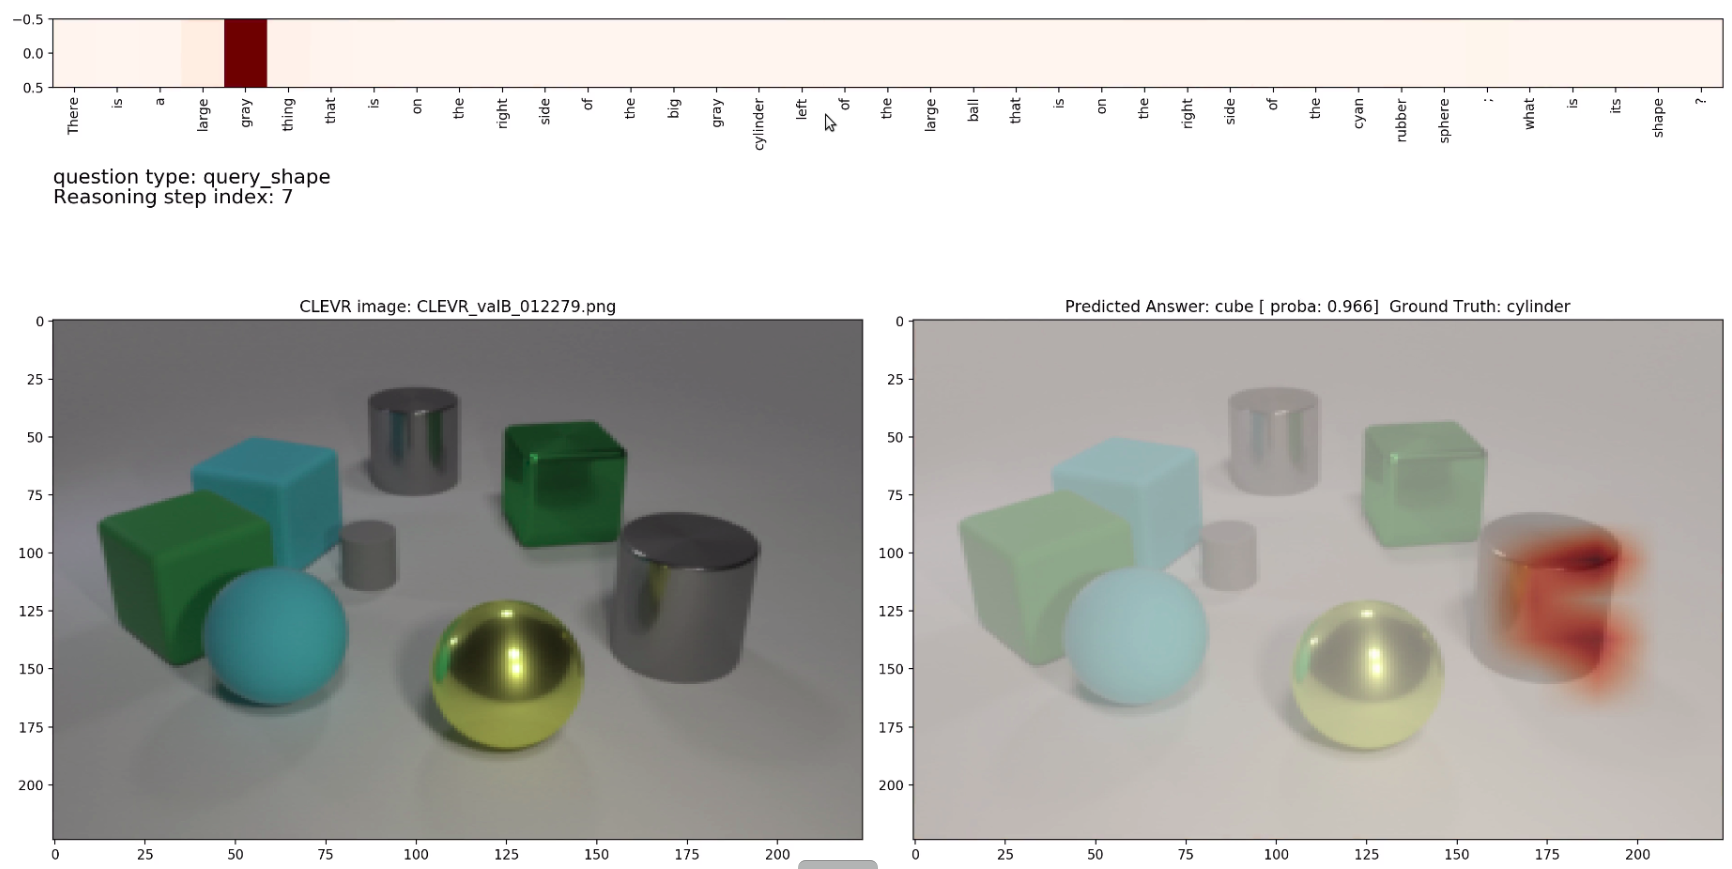
\includegraphics[width=0.60\textwidth]{../img/fail_mac_cogent_b_shape.png}

	
\end{figure}

\begin{description}
	\item[$\bullet$] The question reads as: \textit{There is a large gray thing that is on the right side of the big gray cylinder left of the large ball that is on the right side if the cyan rubber sphere; what is its shape? Predicted answer: Cylinder - Truth: Cube}
	
\end{description}



}

\headerbox{References}{name=references, column=1, below=baseline}{
	\small
	\vspace{-8pt}
	\renewcommand{\refname}{}
	\bibliographystyle{alpha}
	\bibliography{../vigil_bibliography}
	\normalsize
	\textsl{}
}

\end{poster}



\end{document}